\PassOptionsToPackage{unicode=true}{hyperref} % options for packages loaded elsewhere
\PassOptionsToPackage{hyphens}{url}
%
\documentclass[]{article}
\usepackage{lmodern}
\usepackage{fullpage}
\usepackage{amssymb,amsmath}
\usepackage{ifxetex,ifluatex}
\ifnum 0\ifxetex 1\fi\ifluatex 1\fi=0 % if pdftex
  \usepackage[T1]{fontenc}
  \usepackage[utf8]{inputenc}
  \usepackage{textcomp} % provides euro and other symbols
\else % if luatex or xelatex
  \usepackage{unicode-math}
  \defaultfontfeatures{Ligatures=TeX,Scale=MatchLowercase}
\fi
% use upquote if available, for straight quotes in verbatim environments
\IfFileExists{upquote.sty}{\usepackage{upquote}}{}
% use microtype if available
\IfFileExists{microtype.sty}{%
\usepackage[]{microtype}
\UseMicrotypeSet[protrusion]{basicmath} % disable protrusion for tt fonts
}{}
\IfFileExists{parskip.sty}{%
\usepackage{parskip}
}{% else
\setlength{\parindent}{0pt}
\setlength{\parskip}{6pt plus 2pt minus 1pt}
}
\usepackage{hyperref}
\hypersetup{
            pdfborder={0 0 0},
            breaklinks=true}
\urlstyle{same}  % don't use monospace font for urls
\usepackage{color}
\usepackage{fancyvrb}
\newcommand{\VerbBar}{|}
\newcommand{\VERB}{\Verb[commandchars=\\\{\}]}
\DefineVerbatimEnvironment{Highlighting}{Verbatim}{commandchars=\\\{\}}
% Add ',fontsize=\small' for more characters per line
\newenvironment{Shaded}{}{}
\newcommand{\AlertTok}[1]{\textcolor[rgb]{1.00,0.00,0.00}{\textbf{#1}}}
\newcommand{\AnnotationTok}[1]{\textcolor[rgb]{0.38,0.63,0.69}{\textbf{\textit{#1}}}}
\newcommand{\AttributeTok}[1]{\textcolor[rgb]{0.49,0.56,0.16}{#1}}
\newcommand{\BaseNTok}[1]{\textcolor[rgb]{0.25,0.63,0.44}{#1}}
\newcommand{\BuiltInTok}[1]{#1}
\newcommand{\CharTok}[1]{\textcolor[rgb]{0.25,0.44,0.63}{#1}}
\newcommand{\CommentTok}[1]{\textcolor[rgb]{0.38,0.63,0.69}{\textit{#1}}}
\newcommand{\CommentVarTok}[1]{\textcolor[rgb]{0.38,0.63,0.69}{\textbf{\textit{#1}}}}
\newcommand{\ConstantTok}[1]{\textcolor[rgb]{0.53,0.00,0.00}{#1}}
\newcommand{\ControlFlowTok}[1]{\textcolor[rgb]{0.00,0.44,0.13}{\textbf{#1}}}
\newcommand{\DataTypeTok}[1]{\textcolor[rgb]{0.56,0.13,0.00}{#1}}
\newcommand{\DecValTok}[1]{\textcolor[rgb]{0.25,0.63,0.44}{#1}}
\newcommand{\DocumentationTok}[1]{\textcolor[rgb]{0.73,0.13,0.13}{\textit{#1}}}
\newcommand{\ErrorTok}[1]{\textcolor[rgb]{1.00,0.00,0.00}{\textbf{#1}}}
\newcommand{\ExtensionTok}[1]{#1}
\newcommand{\FloatTok}[1]{\textcolor[rgb]{0.25,0.63,0.44}{#1}}
\newcommand{\FunctionTok}[1]{\textcolor[rgb]{0.02,0.16,0.49}{#1}}
\newcommand{\ImportTok}[1]{#1}
\newcommand{\InformationTok}[1]{\textcolor[rgb]{0.38,0.63,0.69}{\textbf{\textit{#1}}}}
\newcommand{\KeywordTok}[1]{\textcolor[rgb]{0.00,0.44,0.13}{\textbf{#1}}}
\newcommand{\NormalTok}[1]{#1}
\newcommand{\OperatorTok}[1]{\textcolor[rgb]{0.40,0.40,0.40}{#1}}
\newcommand{\OtherTok}[1]{\textcolor[rgb]{0.00,0.44,0.13}{#1}}
\newcommand{\PreprocessorTok}[1]{\textcolor[rgb]{0.74,0.48,0.00}{#1}}
\newcommand{\RegionMarkerTok}[1]{#1}
\newcommand{\SpecialCharTok}[1]{\textcolor[rgb]{0.25,0.44,0.63}{#1}}
\newcommand{\SpecialStringTok}[1]{\textcolor[rgb]{0.73,0.40,0.53}{#1}}
\newcommand{\StringTok}[1]{\textcolor[rgb]{0.25,0.44,0.63}{#1}}
\newcommand{\VariableTok}[1]{\textcolor[rgb]{0.10,0.09,0.49}{#1}}
\newcommand{\VerbatimStringTok}[1]{\textcolor[rgb]{0.25,0.44,0.63}{#1}}
\newcommand{\WarningTok}[1]{\textcolor[rgb]{0.38,0.63,0.69}{\textbf{\textit{#1}}}}
\usepackage{graphicx,grffile}
\makeatletter
\def\maxwidth{\ifdim\Gin@nat@width>\linewidth\linewidth\else\Gin@nat@width\fi}
\def\maxheight{\ifdim\Gin@nat@height>\textheight\textheight\else\Gin@nat@height\fi}
\makeatother
% Scale images if necessary, so that they will not overflow the page
% margins by default, and it is still possible to overwrite the defaults
% using explicit options in \includegraphics[width, height, ...]{}
\setkeys{Gin}{width=\maxwidth,height=\maxheight,keepaspectratio}
\setlength{\emergencystretch}{3em}  % prevent overfull lines
\providecommand{\tightlist}{%
  \setlength{\itemsep}{0pt}\setlength{\parskip}{0pt}}
\setcounter{secnumdepth}{0}
% Redefines (sub)paragraphs to behave more like sections
\ifx\paragraph\undefined\else
\let\oldparagraph\paragraph
\renewcommand{\paragraph}[1]{\oldparagraph{#1}\mbox{}}
\fi
\ifx\subparagraph\undefined\else
\let\oldsubparagraph\subparagraph
\renewcommand{\subparagraph}[1]{\oldsubparagraph{#1}\mbox{}}
\fi

% set default figure placement to htbp
\makeatletter
\def\fps@figure{htbp}
\makeatother


\title{Neural Prosthesis - Homework 1} 
\date{April 29, 2018}
\author{Johan Medrano (ID 0645241)}

\begin{document}

    
\maketitle



Experiments presented in this report have been conducted using the
\href{https://neuron.yale.edu/neuron/static/docs/neuronpython/}{Python
module interfacing NEURON}.

\hypertarget{influence-of-an-input-noise-on-the-firing-rate-of-a-neuron}{%
\subsection{1. Influence of an input noise on the firing rate of a
neuron}\label{influence-of-an-input-noise-on-the-firing-rate-of-a-neuron}}

The full code related to this section wan be found in the file np1.py.
Only some important parts will be hilighted in this part.

\hypertarget{introduction}{%
\subsubsection{Introduction}\label{introduction}}

The goal here is to demonstrate the linearization of the firing rate due
to the presence of noise in input of a soma. To do this, we will use
three different somas, each using the same Hogkin-Huxley model for the
membrane. To each soma will be connected a current clamp (\emph{IClamp}
in NEURON).

The former one will be stimulated with a simple current step, while the
second and third ones will receive the same current step cumulated with
different Gaussian noises (zero-mean, \emph{0.05nA} and \emph{0.1nA}
standard deviation, respectively).

\hypertarget{a.-model-creation-and-tuning}{%
\subsubsection{A. Model creation and
tuning}\label{a.-model-creation-and-tuning}}

As we are more interested in qualitative results than quantitative ones,
we use NEURON default parameters for our Hodgkin-Huxley model for
simplicity reasons. The diameter, length and axial resistance of the
soma have been changed accordingly to
\href{http://web.mit.edu/neuron_v7.4/nrntuthtml/tutorial/tutA.html}{this
tutorial}.

Therefore, the model parameters are the following : 
\begin{itemize}
 \item \(\bar{g_{Na}} =120\ mS/cm^2\)
 \item \(\bar{g_K} = 36\ mS/cm^2\)
 \item \(\bar{g_L} = 0.3\ mS/cm^2\) 
 \item \(E_{Na} = 50\ mV\) 
 \item \(E_K = -77\ mV\) 
 \item \(E_L = -54.3\ mV\) 
 \item \(C_m = 1\mu f/cm2\) 
 \item \(d = 18.8\mu m\) 
 \item \(L = 18.8\mu m\) 
 \item \(Ra = 123\Omega.cm\) 
 \item \(nseg = 1\)
\end{itemize}

Note that, as the soma is small and we do not care about spatial
accuracy, we only use one segment.

The implementation of the model is shown below. Four different vectors
are used to record the time and reference voltage of each soma.

\begin{Shaded}
\begin{Highlighting}[]
\CommentTok{# Create 3 soma, one for each kind of simulation (1 clean clamp, 2 noisy)}
\NormalTok{soma }\OperatorTok{=}\NormalTok{ [h.Section(name}\OperatorTok{=}\StringTok{'soma}\SpecialCharTok\NormalTok{(i)) }\ControlFlowTok{for}\NormalTok{ i }\KeywordTok{in} \BuiltInTok{range}\NormalTok{(}\DecValTok{3}\NormalTok{)]}

\NormalTok{v_vec }\OperatorTok{=}\NormalTok{ []}
\ControlFlowTok{for}\NormalTok{ s }\KeywordTok{in}\NormalTok{ soma: }
    \CommentTok{# Tune the soma, inserting HH model}
\NormalTok{    s.insert(}\StringTok{'hh'}\NormalTok{)}
    \CommentTok{# Change diameter, length and axial resistance}
\NormalTok{    s.L }\OperatorTok{=} \FloatTok{18.8}
\NormalTok{    s(}\FloatTok{0.5}\NormalTok{).diam }\OperatorTok{=} \FloatTok{18.8}
\NormalTok{    s.Ra }\OperatorTok{=} \FloatTok{123.}
    \CommentTok{# Some output to check the good configuration}
\NormalTok{    h.psection(sec }\OperatorTok{=}\NormalTok{ s)}

    \CommentTok{# Create a vector recording the membrane reversal potential during the simulation }
\NormalTok{    v }\OperatorTok{=}\NormalTok{ h.Vector() }
\NormalTok{    v.record(s(}\FloatTok{0.5}\NormalTok{)._ref_v)}
\NormalTok{    v_vec.append(v)}

\CommentTok{# Get a time vector}
\NormalTok{t_vec }\OperatorTok{=}\NormalTok{ h.Vector()}
\NormalTok{t_vec.record(h._ref_t)}
\end{Highlighting}
\end{Shaded}

Then we set the parameters of the simulation. We evaluate 1,000
different currents values, varying between \emph{0nA} and \emph{0.4nA}.
The duration of the simulation, which is also the duration of the
current step, is set to \(1,000ms\)

\hypertarget{b.-stimulating-the-clamps}{%
\subsubsection{B. Stimulating the
clamps}\label{b.-stimulating-the-clamps}}

Clamps are created and attached to the soma. The current stimuli is not
totally defined before the simulation step. For noisy clamps, we
manually play a serie of current values in the clamp.

The noisy step is generated using the code below. The main concern is to
not overpass 2,000Hz, as stipulated in the assignement (legend of the
image B).

Thus, a noise of 2,000 points (in the case of a 1-second simulation) is
firstly generated using numpy's Gaussian random number generator, with a
predifined standard deviation. We then take the inverse-FFT of the FFT
of this signal, to cast the 2,000-points signal to a \emph{N}-points
signal without adding higher frequencies. Then the noise signal is
scaled and shifted to have a mean of zero and a desired standard
deviation.

Then this signal is added to a simple step with the desired shape.

\begin{Shaded}
\begin{Highlighting}[]
\CommentTok{# Function make_clamp_noisy creates a clamp with a defined amplitude and noise standard }
\CommentTok{# deviation (noise_amp)}
\KeywordTok{def}\NormalTok{ make_step_noisy(amp, noise_amp, delay, duration): }
\NormalTok{    N }\OperatorTok{=} \BuiltInTok{int}\NormalTok{((delay }\OperatorTok{+}\NormalTok{ duration) }\OperatorTok{/}\NormalTok{ h.dt)}
    \CommentTok{# Noise bandwith is limited to 2000Hz}
\NormalTok{    noise0 }\OperatorTok{=}\NormalTok{ np.random.normal(}\FloatTok{0.}\NormalTok{, noise_amp, }\BuiltInTok{int}\NormalTok{( }\DecValTok{2000}\OperatorTok{*}\NormalTok{(delay }\OperatorTok{+}\NormalTok{ duration)}\OperatorTok{*}\FloatTok{1e-3}\NormalTok{))   }
    \CommentTok{# Use fft and ifft to scale the number of points}
\NormalTok{    noise }\OperatorTok{=}\NormalTok{ np.real(scfft.ifft(scfft.rfft(noise0), N))                  }
    \CommentTok{# Rescale the noise}
\NormalTok{    noise }\OperatorTok{=}\NormalTok{ (noise }\OperatorTok{-}\NormalTok{ np.mean(noise)) }\OperatorTok{*}\NormalTok{ noise_amp}\OperatorTok{/}\NormalTok{np.std(noise)                     }

    \CommentTok{# Create a clean clamp}
\NormalTok{    clean_step }\OperatorTok{=}\NormalTok{ np.array(}
\NormalTok{        [}\DecValTok{0} \ControlFlowTok{if}\NormalTok{ t }\OperatorTok{<}\NormalTok{ delay }\ControlFlowTok{else}\NormalTok{ amp }\ControlFlowTok{for}\NormalTok{ t }\KeywordTok{in}\NormalTok{ np.linspace(}\DecValTok{0}\NormalTok{, delay }\OperatorTok{+}\NormalTok{ duration, N)])}

    \CommentTok{#print("mean %f; std %f"%(np.mean(noise), np.std(noise)))}
    \ControlFlowTok{return}\NormalTok{ noise }\OperatorTok{+}\NormalTok{ clean_step}
\end{Highlighting}
\end{Shaded}

\hypertarget{c.-counting-spikes}{%
\subsubsection{C. Counting spikes}\label{c.-counting-spikes}}

The next step is to create a function to automatically count the
neuronal spikes during the stimulation, to be able to record the firing
rate for different stimulation currents. We have many different ways to
do so, but the idea is to be able to accurately distinguish the spikes
from the voltage waves appearing for a current under the firing current
threshold.

Here, we compute the time first-order derivative of the voltage,
\(\frac{dV}{dt}\). Then, we try to find a significant increase of the
reversal potential, such as \(\frac{dV}{dt}(t) > threshold\). To be sure
to count the spike only once, we just count the point \(t^*\) such as
\(\frac{dV}{dt}(t^*) \approx threshold\) during an increase of the
potential. This point is found by making a linear interpolation : we
find \(t\) such as \(\frac{dV}{dt}(t) < threshold\) and
\(\frac{dV}{dt}(t + \delta t) > threshold\), and we interpolate
\(t^* = \frac{t + (t+\delta t)}{2}\).

By using experimental parameter fitting, we found that a threshold of
\emph{85 mV/ms} was a good value, well discriminative and counting all
the spike for a input current under \emph{0.4 nA}. This parameter will
be use for the following parts.

\begin{Shaded}
\begin{Highlighting}[]
\CommentTok{# Function get_spikes_count counts the number of spikes }
\KeywordTok{def}\NormalTok{ get_spikes_count(v_vec, t_vec, thresh}\OperatorTok{=}\DecValTok{25}\NormalTok{): }
\NormalTok{    dv_vec }\OperatorTok{=}\NormalTok{ [(v_vec[i}\OperatorTok{+}\DecValTok{1}\NormalTok{]}\OperatorTok{-}\NormalTok{v_vec[i])}\OperatorTok{/}\NormalTok{(t_vec[i}\OperatorTok{+}\DecValTok{1}\NormalTok{]}\OperatorTok{-}\NormalTok{t_vec[i]) }\ControlFlowTok{for}\NormalTok{ i }\KeywordTok{in} \BuiltInTok{range}\NormalTok{(}\BuiltInTok{len}\NormalTok{(t_vec) }\OperatorTok{-} \DecValTok{1}\NormalTok{)]}
    \CommentTok{# dt_vec = [(t_vec[i] + t_vec[i+1])/2 for i in range(len(t_vec) - 1)]}
    \CommentTok{# plt.plot(dt_vec, dv_vec)}
    \CommentTok{# plt.show()}
\NormalTok{    spikes_count }\OperatorTok{=}\NormalTok{ np.}\BuiltInTok{sum}\NormalTok{(}
\NormalTok{        [dv_vec[i]}\OperatorTok{<}\NormalTok{thresh }\KeywordTok{and}\NormalTok{ dv_vec[i}\OperatorTok{+}\DecValTok{1}\NormalTok{]}\OperatorTok{>}\NormalTok{thresh }\ControlFlowTok{for}\NormalTok{ i }\KeywordTok{in} \BuiltInTok{range}\NormalTok{(}\BuiltInTok{len}\NormalTok{(dv_vec) }\OperatorTok{-} \DecValTok{1}\NormalTok{)])}
    
    \CommentTok{# The spikes count can be converted in Hertz, and is Hertz for duration = 1000}
    \ControlFlowTok{return}\NormalTok{ spikes_count}
\end{Highlighting}
\end{Shaded}

\hypertarget{d.-putting-everything-together}{%
\subsubsection{D. Putting everything
together}\label{d.-putting-everything-together}}

The code section below presents the full loop used generate data for
differents current. Clamps are firstly configured with the current value
of the loop, then the simulation is ran and voltages are recorded for
each soma. After the loop, voltages are post-processed to get the number
of spikes, which is also the firing rate in Hertz when the simulation
duration is \emph{1 sec.}.

\begin{Shaded}
\begin{Highlighting}[]
\NormalTok{voltages }\OperatorTok{=}\NormalTok{[[],[],[]]}
\CommentTok{# Loop other all the current steps}
\ControlFlowTok{for}\NormalTok{ current }\KeywordTok{in}\NormalTok{ np.linspace(min_curr, max_curr, res): }
    \CommentTok{# Make a step with 2 different noises for this particular current }
\NormalTok{    v_05 }\OperatorTok{=}\NormalTok{ make_step_noisy(current,}\FloatTok{0.05}\NormalTok{, delay, duration)}
\NormalTok{    v_1 }\OperatorTok{=}\NormalTok{ make_step_noisy(current,.}\DecValTok{1}\NormalTok{, delay, duration) }

    \CommentTok{# Assign it to the vector played in amp}
    \ControlFlowTok{for}\NormalTok{ i }\KeywordTok{in} \BuiltInTok{range}\NormalTok{(}\BuiltInTok{len}\NormalTok{(v_05)):}
\NormalTok{        clamp_vec[}\DecValTok{0}\NormalTok{].x[i] }\OperatorTok{=}\NormalTok{ v_05[i]}
\NormalTok{        clamp_vec[}\DecValTok{1}\NormalTok{].x[i] }\OperatorTok{=}\NormalTok{ v_1[i]}

    \CommentTok{# Configure the clean clamp}
\NormalTok{    stim_clean.amp }\OperatorTok{=}\NormalTok{ current}

    \CommentTok{# Run the simulation }
\NormalTok{    h.run() }

    \CommentTok{# Store the voltages records}
    \ControlFlowTok{for}\NormalTok{ i }\KeywordTok{in} \BuiltInTok{range}\NormalTok{(}\BuiltInTok{len}\NormalTok{(voltages)): }
\NormalTok{        c }\OperatorTok{=}\NormalTok{ h.Vector() }
\NormalTok{        c.copy(v_vec[i])}
\NormalTok{        voltages[i].append(c)}


\NormalTok{spikes_count }\OperatorTok{=}\NormalTok{ [[], [], []]}
\CommentTok{# Count the spikes for each voltage recorded}
\ControlFlowTok{for}\NormalTok{ i }\KeywordTok{in} \BuiltInTok{range}\NormalTok{(}\BuiltInTok{len}\NormalTok{(spikes_count)): }
    \ControlFlowTok{for}\NormalTok{ c }\KeywordTok{in} \BuiltInTok{range}\NormalTok{(res): }
\NormalTok{        spikes_count[i].append(get_spikes_count(voltages[i][c], t_vec)) }
\end{Highlighting}
\end{Shaded}

\hypertarget{e.-results-and-discussion}{%
\subsubsection{E. Results and
discussion}\label{e.-results-and-discussion}}

The obtained frequency-current curve under different noise conditions is
presented below. We can see that the Gaussian noise has the effect of
linearizing the behaviour of the soma. The discontinuitie of the current
threshold (around \emph{0.07 nA}) observed on the blue curve, obtain
without noise, is replaced by a curve with a continuous mean, as
observed on the orange and green curves. The standard deviation of the
noise, which determines its ``amplitude'', makes the curve be more
linear by giving higher fire rate values for the smaller currents.

It is important to notice that the way of calculating the firing rate is
not totally correct, which explains the values of \emph{1 Hz} observed
on the blue curve, before the threshold : only one spike has been
counted on the period, so the firing rate has been extrapolated to be
\emph{1 Hz}.

Note also that the firing rate on the orange and green curves in noisy.
This is due to the limited time of the simulation, and the potential
bias in the data generated by the random number generator.

\begin{figure}
\centering
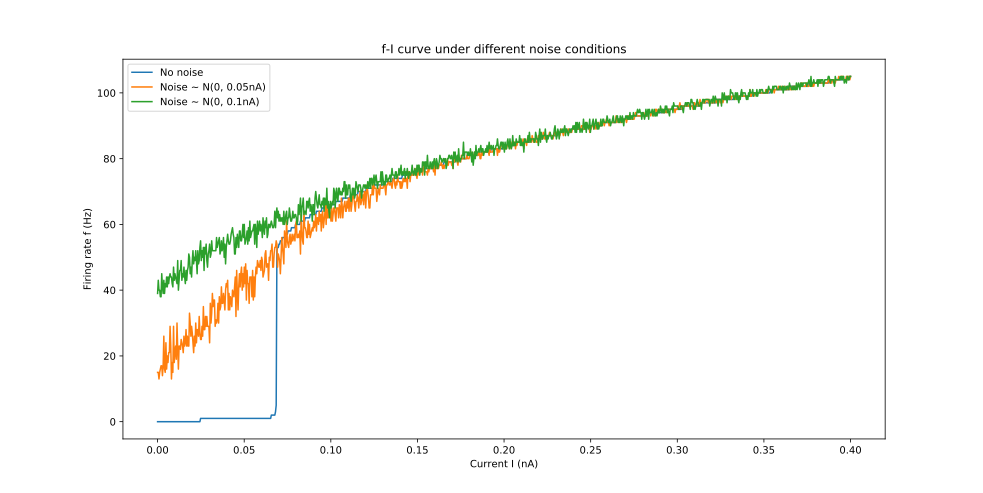
\includegraphics{f-I_under_noise.png}
\caption{f-I curve under different noise conditions}
\end{figure}

\newpage

\hypertarget{influence-of-the-myelin-on-the-conduction-speed-of-an-axon}{%
\subsection{2. Influence of the myelin on the conduction speed of an
axon}\label{influence-of-the-myelin-on-the-conduction-speed-of-an-axon}}

The full code related to this section wan be found in the file np2.py.
Only some important parts will be hilighted in this document.

\hypertarget{introduction-1}{%
\subsubsection{Introduction}\label{introduction-1}}

In this part, the goal is to hilight the changement of behaviour of an
axon, depending on the presence or not of myelin. The idea is put in
evidence that the saltatory conduction of the action potential in the
myelinated axon makes the conduction speed vary linearly with the
diameter of the axon, while its vary proportionnaly to the square root
of the diameter for unmyelinated axons. This is an important property
making the communications faster between neurons.

Hence, to investigate this, we measure the conduction speed of both
myelinated and unmyelinated axons for different diameters. Using linear
regression, we show the correlation between diameter and conduction
speed.

\hypertarget{a.-myelinated-and-unmyelinated-axons-models}{%
\subsubsection{A. Myelinated and unmyelinated axons
models}\label{a.-myelinated-and-unmyelinated-axons-models}}

The dimension of the axons are given in the subject : axons have a total
length of \emph{1.504 mm}, and a diameter varying betweend \emph{1 µm}
and \emph{9 µm}.

\hypertarget{myelinated-axon-model}{%
\paragraph{Myelinated axon model}\label{myelinated-axon-model}}

The myelinated axon model is composed of 7 nodes : 4 Ranvier nodes, and
3 internodal segments.

The Ranvier nodes are the part of the axon without myelin, thus, their
membrane reversal potential is modeled by an Hodgkin-Huxley model. Model
parameters are the same as the one presented in Part 1., for the
modelisation of the soma's membrane, because the quantitative results
are not our main focus. The length of Ranvier nodes is set to \emph{1
µm}.

The internodal segments are the myelinated parts. Myelin works as an
insulator, so we modeled it with a passive channel with a infinite
resistivity, so zero conductivity. We can find in
\href{https://pdfs.semanticscholar.org/a622/57ca2a4024a2165cad8384df388f16208f31.pdf}{this
thesis} (page 30) that the value of resistivity for myelin is on the
scale of \emph{MΩ}. Even if we are not modeling their frog axon, this
gaves an idea of scale and justifies the negligeable error done by
setting the membrane conductivity to \emph{0.0 S/cm2}. Its Nernst
potential has been set to \emph{-65mV}, after experimental parameter
fitting.\\
The length of the internodal segments is set to \emph{500 µm}.

We create a function building an axon with a desired diameter and number
of segments for each node, as presented below.

\begin{Shaded}
\begin{Highlighting}[]
\CommentTok{# Function make_myelinated_axon creates an axon with myelin}
\KeywordTok{def}\NormalTok{ make_myelinated_axon(diameter, nseg}\OperatorTok{=}\DecValTok{3}\NormalTok{, innode_len}\OperatorTok{=}\DecValTok{500}\NormalTok{, }
\NormalTok{        ranvier_len}\OperatorTok{=}\DecValTok{1}\NormalTok{, n_nodes}\OperatorTok{=}\DecValTok{4}\NormalTok{, n_innode}\OperatorTok{=}\DecValTok{3}\NormalTok{, tag}\OperatorTok{=}\VariableTok{None}\NormalTok{):}
    \ControlFlowTok{if}\NormalTok{ tag }\KeywordTok{is} \VariableTok{None}\NormalTok{: }
\NormalTok{        tag }\OperatorTok{=}\NormalTok{ np.random.randint(}\DecValTok{0}\NormalTok{,}\DecValTok{9}\NormalTok{)}
\NormalTok{    axon }\OperatorTok{=}\NormalTok{ []}
    
    \ControlFlowTok{for}\NormalTok{ i }\KeywordTok{in} \BuiltInTok{range}\NormalTok{(n_innode }\OperatorTok{+}\NormalTok{ n_nodes): }

        \ControlFlowTok{if}\NormalTok{ i }\OperatorTok{%} \DecValTok{2} \OperatorTok{==} \DecValTok{0}\NormalTok{: }
            \CommentTok{# Create a Ranvier Node }
\NormalTok{            r }\OperatorTok{=}\NormalTok{ h.Section(name}\OperatorTok{=}\StringTok{'ranvier}\SpecialCharTok{%d%d}\StringTok{'}\OperatorTok{%}\NormalTok{(tag,i))}
            \CommentTok{# Configure the section }
\NormalTok{            r(}\FloatTok{0.5}\NormalTok{).diam }\OperatorTok{=}\NormalTok{ diameter}
\NormalTok{            r.nseg }\OperatorTok{=}\NormalTok{ nseg}
\NormalTok{            r.Ra }\OperatorTok{=} \FloatTok{123.}
\NormalTok{            r.L }\OperatorTok{=}\NormalTok{ ranvier_len}

            \CommentTok{# A Ranvier node is a scection with a HH model}
\NormalTok{            r.insert(}\StringTok{'hh'}\NormalTok{)}

            \ControlFlowTok{if}\NormalTok{ i }\OperatorTok{>} \DecValTok{0}\NormalTok{: }
                \CommentTok{# Connect it to the previous element}
\NormalTok{                r.}\ExtensionTok{connect}\NormalTok{(axon[}\OperatorTok{-}\DecValTok{1}\NormalTok{](}\DecValTok{1}\NormalTok{))}
\NormalTok{            axon.append(r)}
            
        \ControlFlowTok{if}\NormalTok{ i }\OperatorTok{%} \DecValTok{2} \OperatorTok{==} \DecValTok{1}\NormalTok{: }
            \CommentTok{# Create a section surrounded by myelin }
\NormalTok{            m }\OperatorTok{=}\NormalTok{ h.Section(name}\OperatorTok{=}\StringTok{'myelin}\SpecialCharTok{%d%d}\StringTok{'}\OperatorTok{%}\NormalTok{(tag,i))}
            \CommentTok{# Configure the section }
\NormalTok{            m(}\FloatTok{0.5}\NormalTok{).diam }\OperatorTok{=}\NormalTok{ diameter}
\NormalTok{            m.nseg }\OperatorTok{=}\NormalTok{ nseg}
\NormalTok{            m.Ra }\OperatorTok{=} \FloatTok{123.}
\NormalTok{            m.L }\OperatorTok{=}\NormalTok{ innode_len}

            \CommentTok{# Insert a passive channel }
\NormalTok{            m.insert(}\StringTok{'pas'}\NormalTok{)}
            \CommentTok{# Our assumption is the myelin is totally insulator}
\NormalTok{            m.g_pas }\OperatorTok{=} \FloatTok{0.000}
\NormalTok{            m.e_pas }\OperatorTok{=} \DecValTok{-65}

            \CommentTok{# Connect it to the previous element}
\NormalTok{            m.}\ExtensionTok{connect}\NormalTok{(axon[}\OperatorTok{-}\DecValTok{1}\NormalTok{](}\DecValTok{1}\NormalTok{))}
\NormalTok{            axon.append(m)  }

    \ControlFlowTok{return}\NormalTok{ axon}
\end{Highlighting}
\end{Shaded}

\hypertarget{unmyelinated-axon-model}{%
\paragraph{Unmyelinated axon model}\label{unmyelinated-axon-model}}

The model for the unmyelinated axon is quite simpler : it only constists
in a long section for which the reversal potential is modeled by an
Hodkin-Huxley model. Parameters used for the membrane model are the same
as the ones used above for the Ranvier node : as we want to show that
myelin covering parts of the axon (uncovered parts are the Ranvier
nodes) makes the conduction behave differently, the base models of the
axon's membrane have to be the same.

We create a function to create an unmyelinated axon with a desired
diameter and number of segments using the Ranvier node part of the above
function.

\hypertarget{b.-getting-the-spike-time-to-compute-the-conduction-speed}{%
\subsubsection{B. Getting the spike time to compute the conduction
speed}\label{b.-getting-the-spike-time-to-compute-the-conduction-speed}}

During the simulation, we will record the potential for each segment of
the two axons. The location of each record will be known, thus, only the
travel time of the action potential is required to compute its speed.

We tried several methods to get the time at which the action potential
arrived at a specific location, and arbitrarly kept the one presenting
the best results. We compute the second order discrete derivative of the
recorded potential, and find the first peak. This peak happens when the
reversal potential has the highest acceleration.

Using this method the rising time due to the capacitive effect of the
membrane have a small effect on the results. The motivation is that the
capacitance effect will probably already have an effect on the
conduction and will show up at an higher scale, so it does not have to
be counted in the measures.

The function computing the time of the spikes is presented below.

\begin{Shaded}
\begin{Highlighting}[]
\CommentTok{# Function get_spike_time gets the time at which the derivative  }
\KeywordTok{def}\NormalTok{ get_spike_time(v_vec, t_vec):}
    \CommentTok{# First order derivative}
\NormalTok{    dt_vec }\OperatorTok{=}\NormalTok{ [(t_vec[i] ) }\ControlFlowTok{for}\NormalTok{ i }\KeywordTok{in} \BuiltInTok{range}\NormalTok{(}\BuiltInTok{len}\NormalTok{(t_vec) }\OperatorTok{-} \DecValTok{1}\NormalTok{)]}
\NormalTok{    dv_vec }\OperatorTok{=}\NormalTok{ [(v_vec[i}\OperatorTok{+}\DecValTok{1}\NormalTok{]}\OperatorTok{-}\NormalTok{v_vec[i])}\OperatorTok{/}\NormalTok{(t_vec[i}\OperatorTok{+}\DecValTok{1}\NormalTok{]}\OperatorTok{-}\NormalTok{t_vec[i]) }\ControlFlowTok{for}\NormalTok{ i }\KeywordTok{in} \BuiltInTok{range}\NormalTok{(}\BuiltInTok{len}\NormalTok{(t_vec) }\OperatorTok{-} \DecValTok{1}\NormalTok{)]}

    \CommentTok{# Second order derivative}
\NormalTok{    dv2_vec }\OperatorTok{=}\NormalTok{ [(dv_vec[i}\OperatorTok{+}\DecValTok{1}\NormalTok{] }\OperatorTok{-}\NormalTok{ dv_vec[i])}\OperatorTok{/}\NormalTok{(dt_vec[i}\OperatorTok{+}\DecValTok{1}\NormalTok{]}\OperatorTok{-}\NormalTok{dt_vec[i])}
                   \ControlFlowTok{for}\NormalTok{ i }\KeywordTok{in} \BuiltInTok{range}\NormalTok{(}\BuiltInTok{len}\NormalTok{(dt_vec) }\OperatorTok{-} \DecValTok{1}\NormalTok{)]}
\NormalTok{    dt2_vec }\OperatorTok{=}\NormalTok{ [(dt_vec[i]) }\ControlFlowTok{for}\NormalTok{ i }\KeywordTok{in} \BuiltInTok{range}\NormalTok{(}\BuiltInTok{len}\NormalTok{(dt_vec) }\OperatorTok{-} \DecValTok{1}\NormalTok{)]}

    \ControlFlowTok{return}\NormalTok{ dt2_vec[np.argmax(dv2_vec)]}
\end{Highlighting}
\end{Shaded}

\hypertarget{c.-simulation-loop-and-linear-regression}{%
\subsubsection{C. Simulation loop and linear
regression}\label{c.-simulation-loop-and-linear-regression}}

The idea is to evaluate the travel speed for different values of
diameter, and then use linear regression to fit two differents model on
our data.

A current clamp is attached to one extremity of each axon. After \emph{1
ms}, a strong current pulse of \emph{6 nA} is set during \emph{2 ms}. We
measure the travel time as the time between the appearance of the spike
on the first segment and the arrival at the end of the axon, on the last
segment. As the total length if the axon is known, we can easily get the
mean travel speed, which is recorded for each axon diameter. We iterate
over 500 values of diameters between \emph{1 µm} and \emph{9 µm}.

The myelinated axon is build using 15 segments per sections, for a total
of 105 segments. The unique section of the unmyelinated axon has been
defined into the same amount of segments. The core of the loop does not
present a real interest and is not included in this report.

\hypertarget{appartuxe9-linear-regression}{%
\paragraph{Apparté : linear
regression}\label{appartuxe9-linear-regression}}

We then use linear regression with L2 regularisation to find a model
\(\Phi(\textbf{x})\ \textbf{w}\) minimizing the Least Square Error with
our data, i.e. :
\[\textbf{w}^* = argmin_\textbf{w}\ LSE_{L2} = argmin_\textbf{w}\ ||\textbf{y} - \Phi(\textbf{x}) \textbf{w}||^2 + \lambda\Phi(\textbf{x})^T \Phi(\textbf{x})\]

where \(\textbf{y}\) is a vector of speed values and \(\textbf{x}\) a
vector of diameters.\(\Phi(x)\) is the design matrix, thus
\(\Phi(\textbf{x}) = [1\ \textbf{x}]\) if we want to regress a line, and
\(\Phi(\textbf{x}) = [1\ \sqrt{\textbf{x}}]\) if we regress a model
varying with the square root of x. \(\lambda\) is a regularization term
used to avoid overfitting.

The optimal solution of this problem is :
\[ \textbf{w}^* = (\Phi(\textbf{x})^T\Phi(\textbf{x}) + \lambda.I)^{-1}\Phi(\textbf{x})^T \textbf{y}\]

For inference, our model will then be either \(y = x.w_1 + w_0\) or
\(y = \sqrt{x}.w_1 + w_0\), depending on the design matrix used. The
code preforming these operations is shown below.

For practical reasons, the square-root kernel used in the linear
regression of the unmyelinated axon has been shifted by 1, and is
\(\sqrt{x - 1}\). The motivation is to make the square-root be 0 at the
first simulation step, because the curve better fits the data and this
optimization is beyond the scope of the linear regression method.

\begin{Shaded}
\begin{Highlighting}[]
\CommentTok{# Function linreg_2params performs linear regression with a 2-columns design matrix }
\CommentTok{# parametered by a kernel}
\KeywordTok{def}\NormalTok{ linreg_2params(x, y, kernel, lambda_l2}\OperatorTok{=}\FloatTok{1e-3}\NormalTok{): }
    \ControlFlowTok{assert}\NormalTok{(}\BuiltInTok{callable}\NormalTok{(kernel))}
\NormalTok{    phi }\OperatorTok{=}\NormalTok{ np.array([[}\DecValTok{1}\NormalTok{, kernel(v)] }\ControlFlowTok{for}\NormalTok{ v }\KeywordTok{in}\NormalTok{ x])}
\NormalTok{    w }\OperatorTok{=}\NormalTok{ np.dot(np.dot(}
\NormalTok{            np.linalg.pinv(np.dot(phi.transpose(), phi) }\OperatorTok{+}\NormalTok{ lambda_l2 }\OperatorTok{*}\NormalTok{ np.eye(}\DecValTok{2}\NormalTok{)), }
\NormalTok{            phi.transpose()), y)}
    \ControlFlowTok{return}\NormalTok{ w}

\CommentTok{# Model parameters - Optimum of LSE with L2 }
\NormalTok{w_myelinated }\OperatorTok{=}\NormalTok{ linreg_2params(diams, speeds_1, }\KeywordTok{lambda}\NormalTok{ x:x)}
\NormalTok{w_unmyelinated }\OperatorTok{=}\NormalTok{ linreg_2params(diams, speeds_2, }\KeywordTok{lambda}\NormalTok{ x: np.sqrt(x}\DecValTok{-1}\NormalTok{))}

\CommentTok{# Inference models}
\NormalTok{speed_myelinated_reg }\OperatorTok{=} \KeywordTok{lambda}\NormalTok{ x : w_myelinated[}\DecValTok{0}\NormalTok{] }\OperatorTok{+}\NormalTok{ x }\OperatorTok{*}\NormalTok{ w_myelinated[}\DecValTok{1}\NormalTok{]}
\NormalTok{speed_unmyelinated_reg }\OperatorTok{=} \KeywordTok{lambda}\NormalTok{ x : w_unmyelinated[}\DecValTok{0}\NormalTok{] }\OperatorTok{+}\NormalTok{ np.sqrt(x}\DecValTok{-1}\NormalTok{) }\OperatorTok{*}\NormalTok{ w_unmyelinated[}\DecValTok{1}\NormalTok{]}
\end{Highlighting}
\end{Shaded}

\hypertarget{d.-results-and-discussion}{%
\subsubsection{D. Results and
discussion}\label{d.-results-and-discussion}}

The results obtained and the curves fitted with linear regression are
shown in the figure below. We can see that the curve for the myelinated
is not perfectly linear, but behaves as linear while looked at a large
scale.

The left part of the graph seems strange, because the unmyelinated
conduction appears to be faster than the myelinated one. The author has
no concrete explanation for this phenomena. This can come from a
modeling error in the parameters used for the Hodgkin-Huxley models,
which would not be biologically plausible when connected with the
internodes section in the myelinated axon, resulting in strange
behaviour for small diameters.

However, when the axon diameter is bigger than \emph{3 µm} the
myelinated axon becomes faster, and the gap between the speeds keeps
increasing with the diameter. We can there say that the myelinated axon
provides an higher conduction speed, thanks to saltatory conduction.

The second figure below is showing the results obtained for the subjects
diameters, \emph{1µm}, \emph{4µm} and \emph{9µm}. We can see that the
linear regression seems to be more accurate with these data.

To further confirm the speed-against-diameter model one can build a more
accurate machine learning algorithm in order to find the right model for
the data. The simulation also need to be improved, using real world
parameters to model the axons.

\begin{figure}
\centering
\includegraphics{speed_against_diameter.png}
\caption{Conduction speed against diameter curve for myelinated and
unmyelinated axons, 500 points}
\end{figure}

\begin{figure}
\centering
\includegraphics{speed_against_diameter_1_4_9.png}
\caption{Conduction speed against diameter curve for myelinated and
unmyelinated axons, 1µm, 4µm and 9µm}
\end{figure}

\end{document}
